In this lecture we study the problem of selecting politicians who at the same time represent a voters preferred policies and carry the competencies to get these policies implemented. In the two extreme cases we might have either 
\begin{itemize}
    \item[1.] All politicians are equally competent, but voters disagree on the optimal policy.
    \item[2.] All voters(/politicians) agree on what is the optimal policy but politicians vary in their competence.
\end{itemize}
When considering some mix of these two extremes a tradeoff arises between competence and policy. In particular all voters wants to be represented by someone competent, but differ what policy attitudes they prefer.

\subsection{Model by \cite{mattozzi_right_2018}}
The model is very similar to the regular downsian model. A continuum of citizens with measure 1 vary in their income and are taxed with some rate $\tau$ to provide a public good. Candidates for elections are drawn from the population and have no commitment to their proposals after election. 

Voters are assumed to live in one of $2n +1$ districts, each of which elect a single legislator. The level of $g$ is set independently for each district, but the tax rate is fixed at a single value, so legislators goal is to bargain a high level of expenditures in their own district.

\paragraph{Voters} 
Voters are split in two groups, the "poor/unsuccessful" with income $y_l$ and the "rich/sucessful" with income $y_h = \eta y_l$. Some share $\gamma>1/2$ of voters are poor. 
The voters utility is quasi-linear in preferences over after-tax income and the level of public good provided in their district. I.e.
\begin{equation}
    u_{ij} =(1-\tau) y^i + g(\pi^j \tau \bar{y})
\end{equation}
where $\bar{y}$ is the average income across all voters and $\pi^j$ is the proportion of total revenue $\tau \bar{y}$ that goes to district $j$. From this we see that given any split $\pi^j$ low type citizens prefer a higher tax rate than high type citizens\footnote{See $\partial_{\tau} u_{ij}=-y^i + \pi^j \bar{y} g'(\pi^j \tau \bar{y})$. Thus in optimum 
\begin{equation}
    \tau = \frac{1}{\pi^j \bar{y}} g'^{-1}(\frac{y^i}{\pi^j \bar{y}})
\end{equation}}
Letting $\tau_l^*$ and $\tau_h^*$ denote the preferred tax rates when revenue is split equally between the districts it must be that $\tau_l^* > \tau_h^*$. 

Obviously given a $\tau$ the voters in district $j$ prefers $\pi^j$ to be set as high as possible.

\paragraph{Elections}
Elections are held at the same time across all districts. In each election one low type voter and one high type voter runs, and we assume that voters are distributed such that $\lambda>1/2$ of districts have a majority of low type candidates. Applying the median voter theorem, any district with a majority of poor individual will have a median voter who is also poor who decides the election, and any rich district will have a rich median voter who decides the election.

\paragraph{Legislature}
The legislature might either be majority rich or majority poor depending on the elections. The way legislature works is that they first vote on a tax rate $\tau$ and then bargain for the shares $\pi^j$ that goes to each district.
\\ \\ 
In the bargaining phase we assume that high income individuals are better at bargaining, by the reasoning that if you do well in the private sector you will also do well in the legislature. The abilities of legislators $(a_1, a_2,...,a_N)$ are set such that $a_l=1$ and $a_h = \eta$. The parameter $\gamma$ governs how much ability matters for bargaining, and so the outcome of bargaining is $\pi^{j*}(a_1,a_2,...,a_N|\gamma)$. Now if bargaining ability has no influence the outcome for each district will be $\pi^{j*}(a_1, ...,a_N|\gamma = 0)\rightarrow1/N$, that is districts simply split the revenue equally. We will further assume that $\partial_{a_j} \pi^{j*}\geq 0$ and $\partial_{a_k} \pi^{j*} \leq 0$ for all $j\neq k$. This simply says that higher bargaining ability of the legislator from district $j$ increases the spending in district $j$ won in bargaining, while higher bargaining abilities of legislators from other districts decrease the spending in district $j$.
\\ \\
The core question in this model is then who voters will elect, someone who share their views on the optimal $\tau$ or someone who can bargain a large share of the tax revenue to the home district. Naturally high type voters prefer to vote for a high type candidate, as they can get both low taxes and competent bargaining from the same candidate. Low income voters however face a tradeoff between getting a legislator who votes for higher taxes and one who bargains well. How this plays out depends on the value of $\gamma$:
\begin{itemize}
    \item[1.] if $\gamma = 0$ there os no tradeoff, so poor districts elect poor candidates. Since there is a majority of poor candidates the legislature will be majority poor and select a tax of $\tau_l^*$. This is a fully representative equilibrium as the median voter is low, so is the median legislator and the outcome is in accordance with their preferences.
    \item[2.] if $\gamma$ is sufficiently high, voters concern with electing a competent politician dominates, so all districts select a high type candidate and the legislature implements $\tau_h^*$. In this equilibrium there is no representativeness, as no legislators will be low type even though a majority of voters are. 
    \item[3.] if $\gamma$ is moderate once a majority $n+1$ have elected a low type it is certain that a low type candidate will by the MVT set the tax rate, and the remaining poor districts become free to select a candidate with high bargaining abilities meaning $n$ high type candidates will enter the legislature. In this case the equilibrium is somewhat representative, as the tax rate is set by a low type, but there is a over representation of high type legislators in the legislature and as a consequence the tax rate will be set lower than $\tau_l^*$ in anticipation of bargaining, in which the districts with low type legislators will have to fund some of the high-type districts spending. 
\end{itemize} 

In summary this model predicts a tradeoff between electing competent politicians and getting a high tax rate for low-income individuals in district voting systems. 

\subsection{Empirics \citep{dal_bo_who_2017}}
Using purely descriptive analysis \cite{dal_bo_who_2017} use a dataset with the entire swedish population as well as various special information on politicians and candidates for elections.

This includes information from conscription tests including IQ and in some cases "leadership tests" undertaken with a psychologist.

To not mechanically measure a correlation between being in the "elite" (a politician) and competence they use parents background as a proxy for representation - i.e. if ones parents were regular people, it is fair to assume that one represents this group, and not the "elite" in the legislature (?). 


\begin{SCfigure}[][h]
    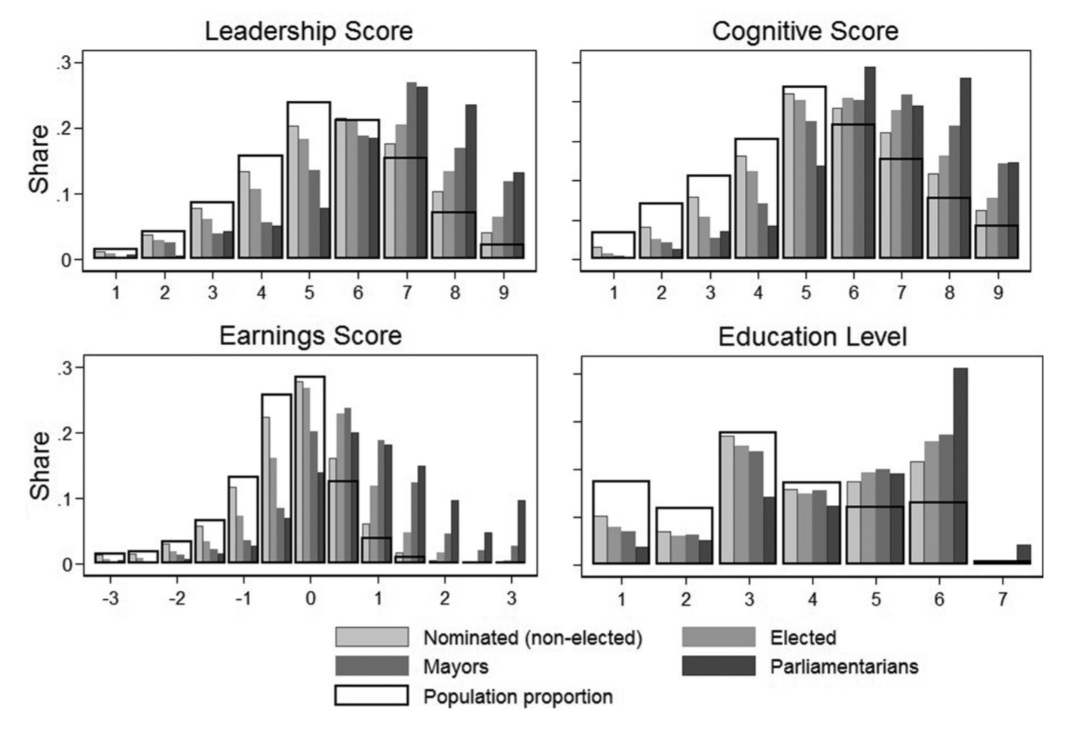
\includegraphics[width=0.6\textwidth]{figures/dal_bo_1.png}
    \caption{\textbf{Results from \cite{dal_bo_who_2017}} The results compares the distribution of various measures of competence with the population distribution of these traits.}    
\end{SCfigure}

The authors find a systematic tendency for politicians to be high competence individuals, with this trend being stronger the higher the office held. This selection is much less pronounced when comparing to parents background. In the sense that the relevant dimension for measuring representation is across generations this suggests that representation issues are not nearly as large as they could have been. In particular it seems that all parties select candidates who themselves are high competence, but tend to favor candidates whose parental background lies in different parts of the income distribution. 

Importantly the lack of relation between parents background and being a politician does not mean that there is no intergenerational persistence in income and abilities etc. Instead the parties have stronger selection for candidates with background lower in the income distribution, evening out the correlation. In other words if your parents are rich you dont have to be very clever to become a politician, but if they're poor you need to be very smart. This selection removes the apparent relation between parents abilities and being a politician.
\\ \\
In summary in Sweden politicians are highly competent compared to the population, but are representative in terms of their background.